%%%%%%%%%%%%%%%%%%%%%%%%%%%%%%%%%%%%%%%%%%%%%%%%%%%%%%%%%%%%%%%%%%%%%%%%%%%%%%%%
\documentclass[twocolumn]{revtex4}

%%%%%%%%%%%%%%%%%%%%%%%%%%%%%%%%%%%%%%%%%%%%%%%%%%%%%%%%%%%%%%%%%%%%%%%%%%%%%%%%
% Note that comments begin with a "%" and are not turned into text in the .pdf
% document.
%%%%%%%%%%%%%%%%%%%%%%%%%%%%%%%%%%%%%%%%%%%%%%%%%%%%%%%%%%%%%%%%%%%%%%%%%%%%%%%%

%%%%%%%%%%%%%%%%%%%%%%%%%%%%%%%%%%%%%%%%%%%%%%%%%%%%%%%%%%%%%%%%%%%%%%%%%%%%%%%%
% Include some extra packages.
%%%%%%%%%%%%%%%%%%%%%%%%%%%%%%%%%%%%%%%%%%%%%%%%%%%%%%%%%%%%%%%%%%%%%%%%%%%%%%%%
\usepackage[]{graphicx}
\usepackage[]{placeins}
%%%%%%%%%%%%%%%%%%%%%%%%%%%%%%%%%%%%%%%%%%%%%%%%%%%%%%%%%%%%%%%%%%%%%%%%%%%%%%%%

%%%%%%%%%%%%%%%%%%%%%%%%%%%%%%%%%%%%%%%%%%%%%%%%%%%%%%%%%%%%%%%%%%%%%%%%%%%%%%%%
\begin{document}

%%%%%%%%%%%%%%%%%%%%%%%%%%%%%%%%%%%%%%%%%%%%%%%%%%%%%%%%%%%%%%%%%%%%%%%%%%%%%%%%
\title{
Predicting the Weather
}

\author{Z.~Goodsell}
\affiliation{Siena College, Loudonville, NY}

\date{\today}

\begin{abstract}
The goal of this project is to predict the weather using the Monte Carlo approach. The Monte Carlo method is a technique in which a large quantity of randomly generated numbers are studied using a probabilistic model to find an approximate solution to a numerical problem that would be difficult to solve by other methods. In problem 1, I had to find the probability that it would rain one and only one day a month when their is a 20 percent chance of rain each day. The probability of this problem analytically is 0.928 percent and using the Monte Carlo approach 0.933 percent. The percent error of between the analytical and Monte Carlo method is 0.511 percent. In problem 2, I had to find the probability odds that it rains at least 8 days in any given month with a 10 percent chance of rain each day. With the Monte Carlo approach, it was found that the probability was 0.784 percent. In problem 3, I was given the following perimeters. Suppose that if it rains one day, the odds of a certain amount of rainfall on that day are, 1 cm - 20 percent, 2 cm - 30 percent, 3 cm - 30 percent, 4 cm - 10 percent, and  5 cm - 10 percent. However the odds of it raining are dependent on if it rained the day before. If it is the first day of the month, there is a 10 percent chance of rain. If it rained 1 day before, but not 2 days before, there is a 20 percent chance of rain.  If it rained both of the 2 days before, but not the 3rd day before, there is a 25 percent chance of rain.  If it rained for the 3 days or more before, there is a 5 percent chance of rain.  Otherwise, there is a 10 percent chance of rain. For problem 3a I had to find the probability that there are at least 10 cm of rain in a given month and I found the probability to be 38.6 percent. For problem 3b I had to create a histogram of the distribution of expected rainfall values and for problem 3c I had to find the average amount of rain in any given months, this was found to be 8cm. Finally, for problem 3d, I had to find the uncertainty of my prediction for the previous problem and this was found to be between 0 cm and 21 cm.
\end{abstract}

\maketitle
%%%%%%%%%%%%%%%%%%%%%%%%%%%%%%%%%%%%%%%%%%%%%%%%%%%%%%%%%%%%%%%%%%%%%%%%%%%%%%%%

%%%%%%%%%%%%%%%%%%%%%%%%%%%%%%%%%%%%%%%%%%%%%%%%%%%%%%%%%%%%%%%%%%%%%%%%%%%%%%%%
\section{Problem 1}
%%%%%%%%%%%%%%%%%%%%%%%%%%%%%%%%%%%%%%%%%%%%%%%%%%%%%%%%%%%%%%%%%%%%%%%%%%%%%%%%
The point of this problem is to find the probability that is would rain one and only one day a month when their is a 20 percent chance of rain each day. To solve this problem analytically we use the following equation. $$(0.2)^1*(0.8)^{(29)}*30*100$$
With this equation the probability was found to be 0.928.

Using the Monte Carlos approach, I started with a function that generated a random number between 0 and 1. If this random number was between 0 and 0.2 its returned a 1, meaning its true and rained, otherwise it returned a 0, meaning its false and didn't rain. Next, I created another function that takes in the previous function and loops it 30 times for the 30 days in the month, each time appending the value returned to a list. If the list equals 1 then 1 is returned as true because it only rained 1 day that month, otherwise it returns 0. Next I took the my second function and looped it 10000 times, adding each 1 returned to a variable. Finally I took the variable and divided it by 10000 to get 0.933.

 
%%%%%%%%%%%%%%%%%%%%%%%%%%%%%%%%%%%%%%%%%%%%%%%%%%%%%%%%%%%%%%%%%%%%%%%%%%%%%%%%
\section{Problem 2}
The point of this problem is to find the probability that it will rain 8 or more days in any given moths with a 10 percent chance of rain each day. Using the Monte Carlos approach, I started with a function that generated a random number between 0 and 1. If this random number was between 0 and 0.1 its returned a 1, meaning its true and rained, otherwise it returned a 0, meaning its false and didn't rain. Next, I created another function that takes in the previous function and loops it 30 times for the 30 days in the month, each time appending the value returned to a list. If the list was equal to or greater then 8, then 1 is returned as true because it rained 8 or more days that month, otherwise it returns 0. Next I took the my second function and looped it 10000 times, adding each 1 returned to a variable. Finally I took the variable and divided it by 10000 to get 0.86. 

%%%%%%%%%%%%%%%%%%%%%%%%%%%%%%%%%%%%%%%%%%%%%%%%%%%%%%%%%%%%%%%%%%%%%%%%%%%%%%%%
\section{Problem 3}
I was given the following perimeters. Suppose that if it rains one day, the odds of a certain amount of rainfall on that day are, 1 cm - 20 percent, 2 cm - 30 percent, 3 cm - 30 percent, 4 cm - 10 percent, and  5 cm - 10 percent. However the odds of it raining are dependent on if it rained the day before. If it is the first day of the month, there is a 10 percent chance of rain. If it rained 1 day before, but not 2 days before, there is a 20 percent chance of rain.  If it rained both of the 2 days before, but not the 3rd day before, there is a 25 percent chance of rain.  If it rained for the 3 days or more before, there is a 5 percent chance of rain.  Otherwise, there is a 10 percent chance of rain.
\subsection{}
The point of this problem is to find the probability that their are at least 10 cm of rain in any given month given the perimeters. The following is in a loop of the number of months you desirer. First I use a loop to generate a list of 30 random numbers from 0 to 1. Next I tested day one against .1 to see if it rained, if true 1 added to a list, otherwise 0 was add. Next I tested to see if it rained day 2, if it did tested day two against .2,  if true 1 added to a list, otherwise 0 was add. If it didn't rain on day 1, day 2 was tested against .1. Now, I tested to see if it rained day 1 and day 2, if it rained both days before day 3 was tested against 0.25. If it only rained the day for it is tested against .2, and if it didn't rain the day before day 3 is tested against .1. Now I start a loop to test days 4 thought 30. The loop starts off by testing if it rained the 3 consecutive days before, if it did the odds of rain are 0.5. If that was false it tests if it rained the 2 consecutive days before, if it did the odds of rain are 0.25. If that was false it tests if it rained the 1 day before, if it did the odds of rain are 0.2. And if that was false, it is testes against 0.1. If the days never finds a true statement 0 is added to a list, otherwise a 1 is added to a list. Now I took the number of days it rained each month and put that into a loop. This loop generated a random number between 0 and 1. If the random number was between 0 and .2 it rained 1 cm, between .2 and .5 it rained 2 cm, between .5 and .8 it rained 3 cm, between .8 and .9 it rained 4 cm, between .9 and 1 it rained 5 cm. The amount it rained more then 9 cm in a certain month is added to a list. Now the list is divided by the number of months, I found a result of 38.6.
\subsection{}
\FloatBarrier
\begin{figure}[h]
\center
    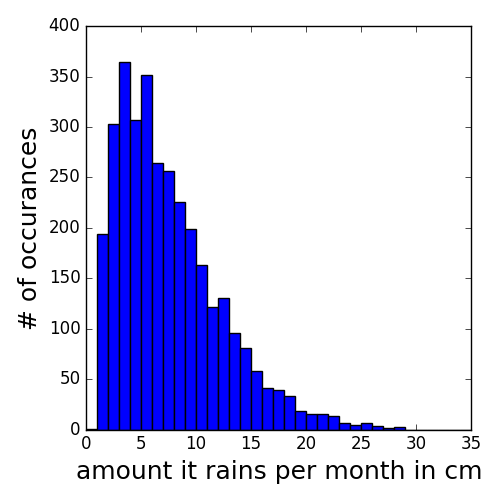
\includegraphics[width=0.45\textwidth]{figure.png}
\end{figure}
\FloatBarrier
\subsection{}
The point of this problem is to find the probability that their are at least 10 cm of rain in any given month given the perimeters. The following is in a loop of the number of months you desirer. First I use a loop to generate a list of 30 random numbers from 0 to 1. Next I tested day one against .1 to see if it rained, if true 1 added to a list, otherwise 0 was add. Next I tested to see if it rained day 2, if it did tested day two against .2,  if true 1 added to a list, otherwise 0 was add. If it didn't rain on day 1, day 2 was tested against .1. Now, I tested to see if it rained day 1 and day 2, if it rained both days before day 3 was tested against 0.25. If it only rained the day for it is tested against .2, and if it didn't rain the day before day 3 is tested against .1. Now I start a loop to test days 4 thought 30. The loop starts off by testing if it rained the 3 consecutive days before, if it did the odds of rain are 0.5. If that was false it tests if it rained the 2 consecutive days before, if it did the odds of rain are 0.25. If that was false it tests if it rained the 1 day before, if it did the odds of rain are 0.2. And if that was false, it is testes against 0.1. If the days never finds a true statement 0 is added to a list, otherwise a 1 is added to a list. Now I took the number of days it rained each month and put that into a loop. This loop generated a random number between 0 and 1. If the random number was between 0 and .2 it rained 1 cm, between .2 and .5 it rained 2 cm, between .5 and .8 it rained 3 cm, between .8 and .9 it rained 4 cm, between .9 and 1 it rained 5 cm. The amount it rained in a  month is added to a list. Now the list is divided by the number of months, I found a result of 8.64. 
\section{}
Once I found the average value, I found the uncertainty on my prediction. I estimate the rainfall to be between 0 cm and 21 cm. I found this by using the percentile function found in numpy with a list of sorted values.

%%%%%%%%%%%%%%%%%%%%%%%%%%%%%%%%%%%%%%%%%%%%%%%%%%%%%%%%%%%%%%%%%%%%%%%%%%%%%%%%
\end{document}
%%%%%%%%%%%%%%%%%%%%%%%%%%%%%%%%%%%%%%%%%%%%%%%%%%%%%%%%%%%%%%%%%%%%%%%%%%%%%%%%
